\documentclass{article}
\usepackage[a4paper]{geometry}
\usepackage[spanish]{babel}
\usepackage{parskip}
\usepackage{setspace}
\usepackage{graphicx}
\usepackage{fancyhdr}
\geometry{total={6in, 9in}}
\usepackage{blindtext} % no sé 
\usepackage{makeidx} % no sé 
\usepackage{lscape}
\usepackage{pdflscape}
\usepackage{fancyhdr}
\usepackage{pdfpages}
\usepackage{rotating}
\usepackage{etoolbox}
\usepackage{listings}
\usepackage{float}
\usepackage{caption}
\usepackage{subcaption}

\lstdefinestyle{customc}{
  language=C++,
  showstringspaces=false,
  basicstyle=\footnotesize\ttfamily,
  keywordstyle=\bfseries\color{green!40!black},
  commentstyle=\itshape\color{purple!40!black},
  identifierstyle=\color{blue},
  stringstyle=\color{orange},
}

\lstset{escapechar=@,style=customc}

\newcommand{\tabitem}{%
  	\usebeamertemplate{itemize item}\hspace*{\labelsep}}
\usepackage[hidelinks]{hyperref}

%HEADRULE

\pagestyle{fancy}
\setlength{\headheight}{30.2pt}
\setlength{\headsep}{30pt}
% INICIO DE PÁGINAS
\begin{document}
\begin{titlepage}
	
	
	\begin{center}
		{\LARGE \textbf{UNIVERSIDAD NACIONAL DE INGENIERÍA}}\\
		\vspace{5 mm}
		{\large \textbf{Facultad de Ingeniería Industrial y de Sistemas}}\\
		\vspace{15.5 mm}
		\begin{figure}[h]
			\centering 
			
\includegraphics[width=0.45\textwidth]{images/CiberSecFIIS.png}
		\end{figure}
		\vspace{4 mm}	
		{\Large \textbf{Informes de exploración de vulnerabilidades en HTB} }\\
		\vspace{5 mm}
		
		\onehalfspacing  % Espaciamiento 1.5
		{\Large \textbf{``{\@De las máquinas: OpenAdmin, Fuse \\Magic, Remote }''} }\\
		
		\singlespacing  % Fin del espaciamiento 1.5
		
		\vspace{4 mm}	

		\vspace{20 mm}
		{\large \textbf{ELABORADO POR:} }\\
		\vspace{10 mm}
		\begin{center}
			\begin{minipage}{0.7\textwidth}
			  \begin{itemize}
				\item \Large Alfonso Suárez, Luis
				\item \Large Mottoccanche Tantaruna, Joseph
				\item \Large Chi Jon, Lau
			  \end{itemize}
			\end{minipage}
		  \end{center}

		\vspace{5 mm}	
	\end{center}

\end{titlepage}


\clearpage
\tableofcontents
\clearpage
% ----------------------------OPENADMIN-----------------------------------
\section{OpenAdmin}
\subsection{Enumeración}

Realizando el escaneo de puertos abiertos encontramos el servicio HTTP en el puerto 80 y SSH, en el puerto 22. El sistema operativo de la máquina observamos que es Linux.
\begin{figure}[H]
	\center
	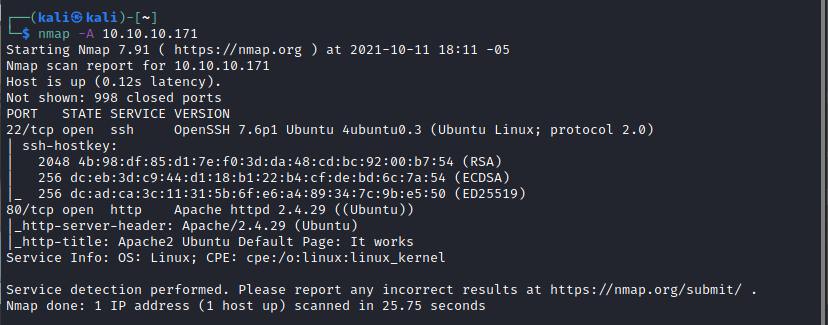
\includegraphics[width=0.8\textwidth]{images/openadmin/1-escaneo.png}
	\caption{Escaneo}
\end{figure}

Accediendo a la página web comprobamos que efectivamente esta máquina está un servidor Apache2. Por lo tanto, hacemos una búsqueda de directorio con dirb, entonramos /artwork/, /music/, y /ona.
\begin{figure}[H]
	\center
	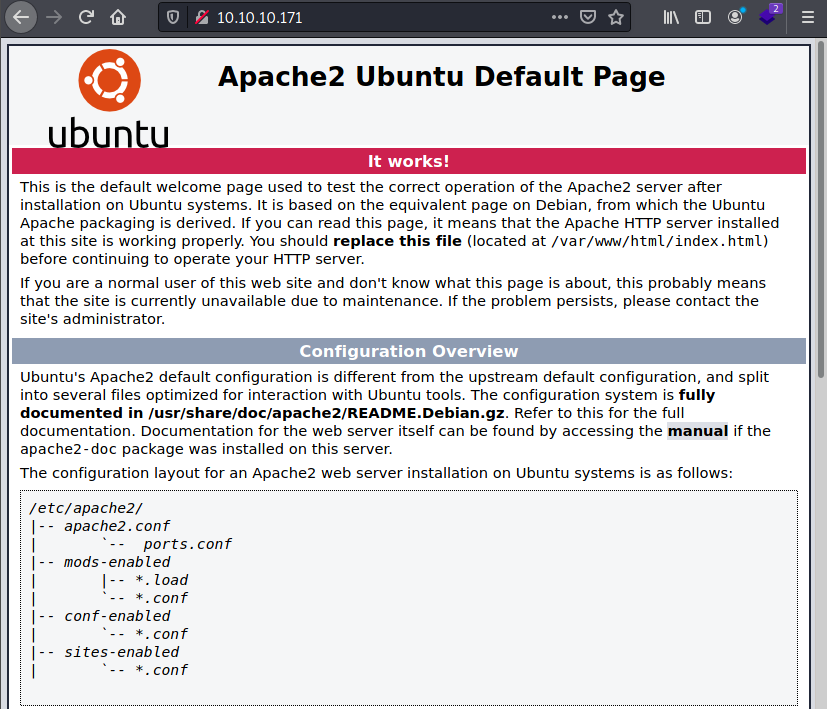
\includegraphics[width=0.8\textwidth]{images/openadmin/2-paginaweb.png}
	\caption{Página Web del puerto 80}
\end{figure}	

Inspeccionando las rutas y su contenido no observamos nada interesante excepto /ona. Observamos que es OpenNetAdmin, googleando encontramos con esta descripción del servicio: “OpenNetAdmin proporciona un inventario administrado de base de datos de su red IP”.
\begin{figure}[H]
	\center
	%\begin{tabular}[c]{cc}
		\begin{subfigure}[c]{\linewidth}
		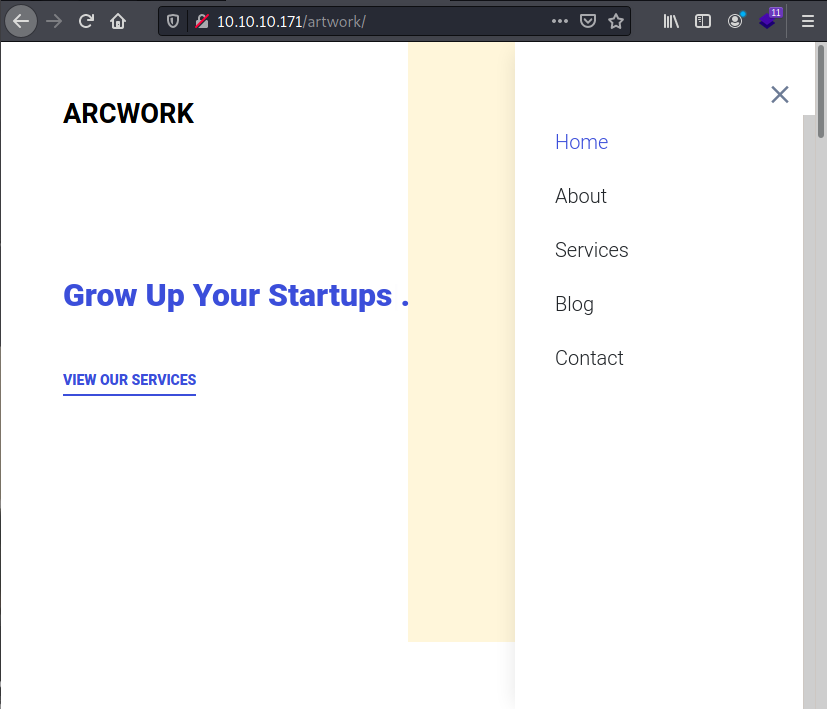
\includegraphics[width=0.5\textwidth]{images/openadmin/3-artwork.png}
		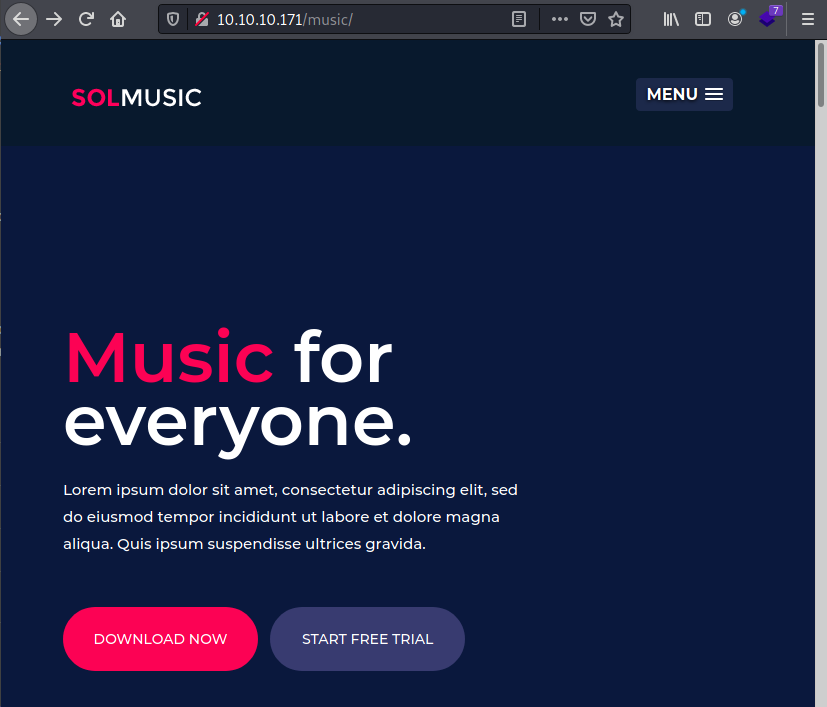
\includegraphics[width=0.5\textwidth]{images/openadmin/4-music.png}
		\end{subfigure}\par\medskip
	%\end{tabular}
	\caption{De izquierda a derecha: /artwork, /music}
\end{figure}

\begin{figure}[H]
	\center
	\begin{subfigure}[c]{\linewidth}
	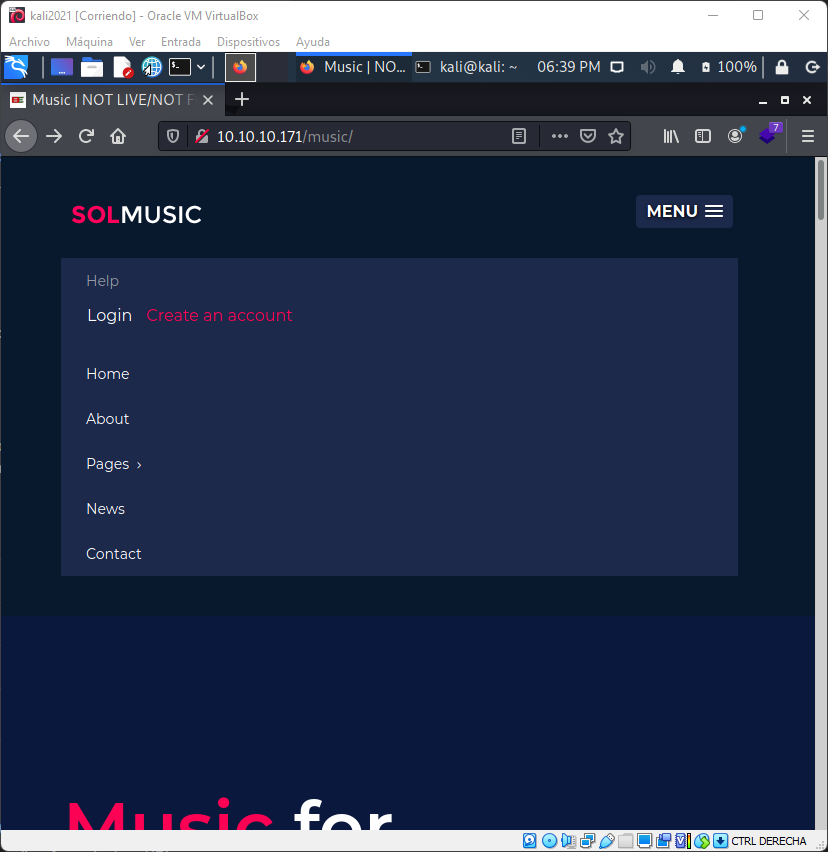
\includegraphics[width=0.5\textwidth]{images/openadmin/4-musicdetalles.png}
	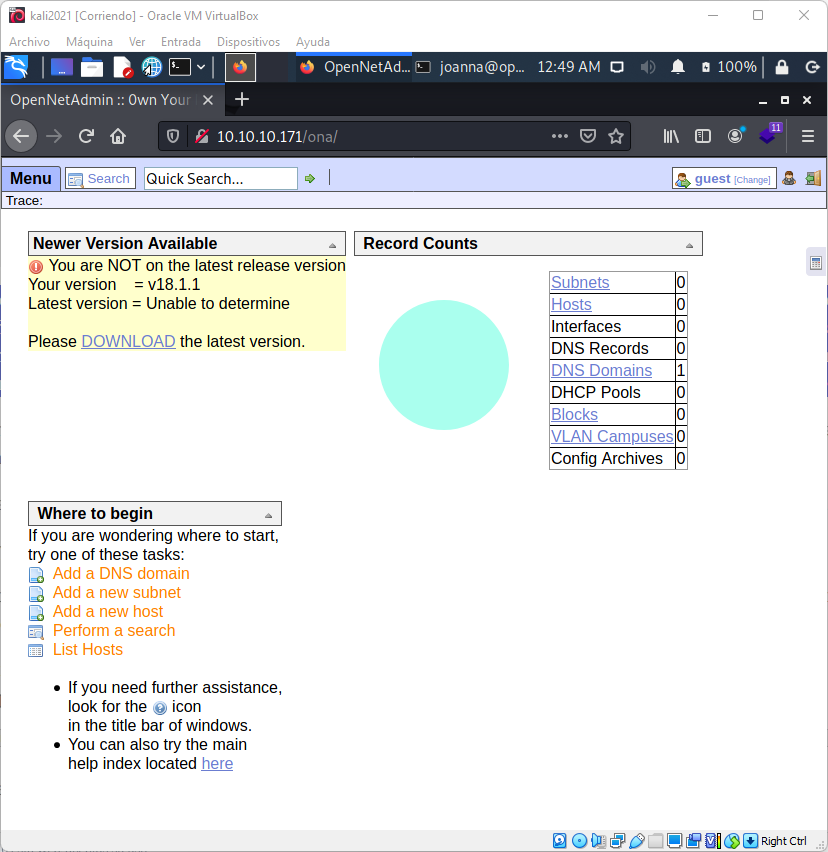
\includegraphics[width=0.5\textwidth]{images/openadmin/5-ona.png}
	\end{subfigure}
	\caption{De izquierda a derecha: /music, /ona}
\end{figure}

Buscando vulnerabilidades de este servicio, observamos en su página que es la versión v18.1.1. Utilizando searchsploit y Google encontramos que tiene una vulnerabilidad por parte de xajax que permite ejecución de código remoto.
\begin{figure}[H]
	\center
	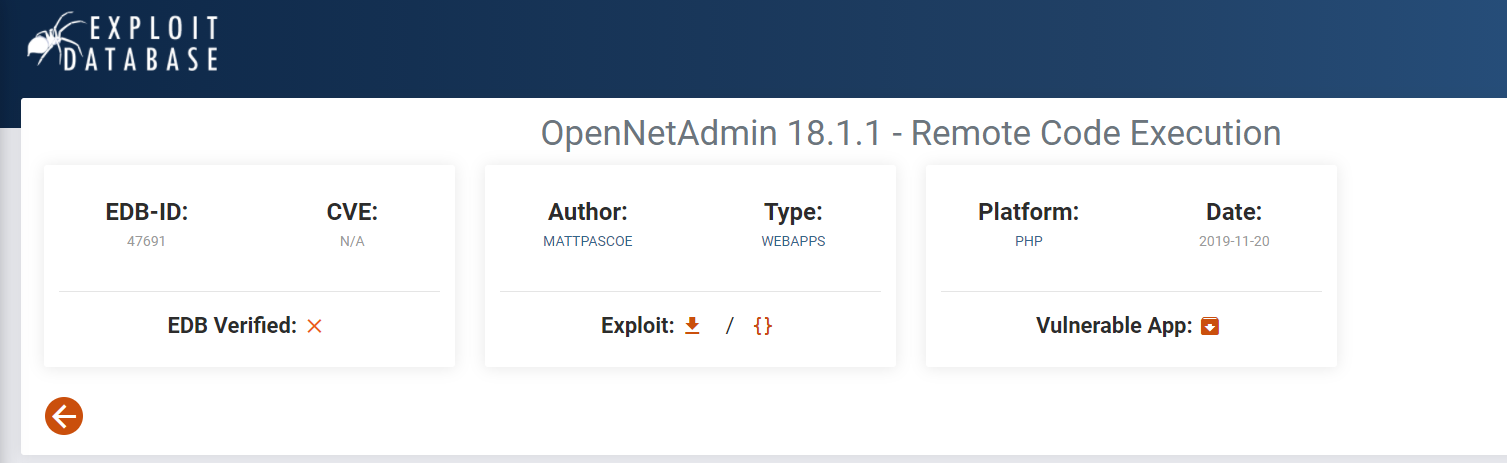
\includegraphics[width=0.8\textwidth]{images/openadmin/6-exploit.png}
	\caption{Exploit del OpenNetAdmin v18.1.1}
\end{figure}

\subsection{Explotación}

Utilizando el script proporcionado logramos obtener acceso al servidor y observamos que somos el usuario www-data.
\begin{figure}[H]
	\center
	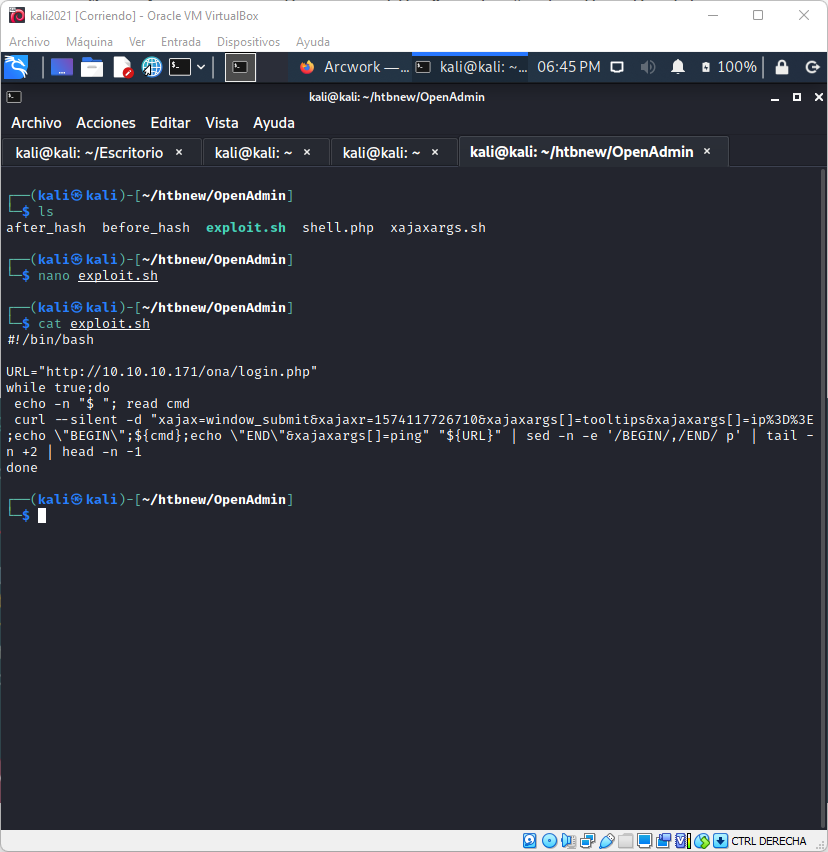
\includegraphics[width=0.8\textwidth]{images/openadmin/7-script.png}
	\caption{Script del exploit}
\end{figure}

\subsubsection{Obtención de Acceso como usuario jimmy}

Inspeccionando los archivos de configuración del servicio ONA, encontramos una credencial. Observamos además que hay dos usuarios jimmy y Joanna.
\begin{figure}[H]
	\center
	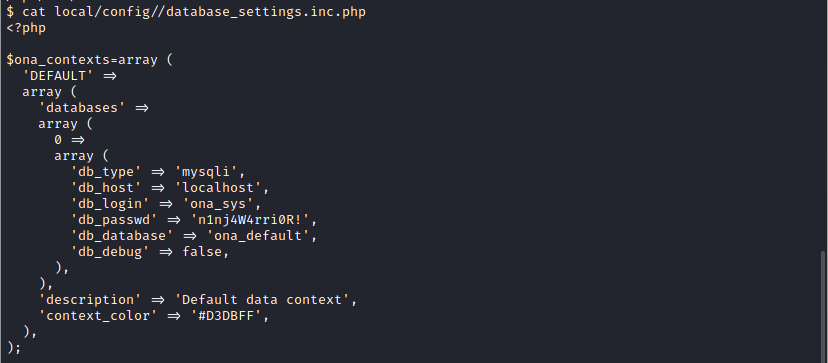
\includegraphics[width=0.8\textwidth]{images/openadmin/8-credencialesjimmy.png}
	\caption{archivo de configuración}
\end{figure}

Además, encontramos que en /var/www hay una carpeta llamada internal que solo puede ser accedida por jimmy.
\begin{figure}[H]
	\center
	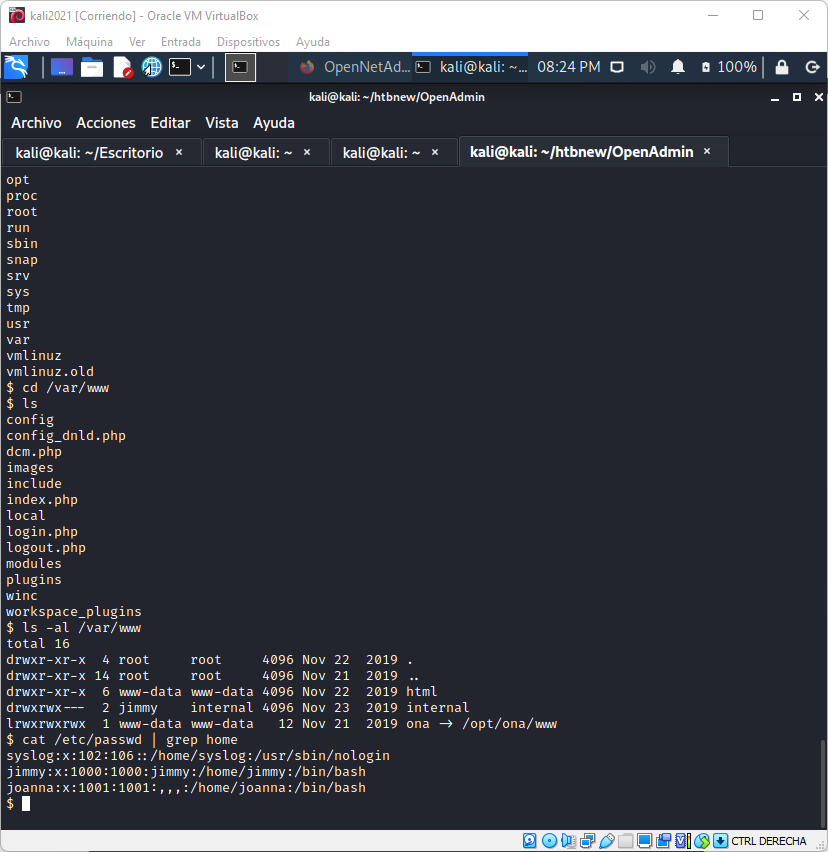
\includegraphics[width=0.8\textwidth]{images/openadmin/9-usuariosycarpetas.png}
	\caption{Usuarios y carpetas en /var/www}
\end{figure}

Procedemos a probar la contraseña encontrada anteriormente mediante ssh y vemos que funciona para el usuario jimmy y no joanna.
\begin{figure}[H]
	\center
	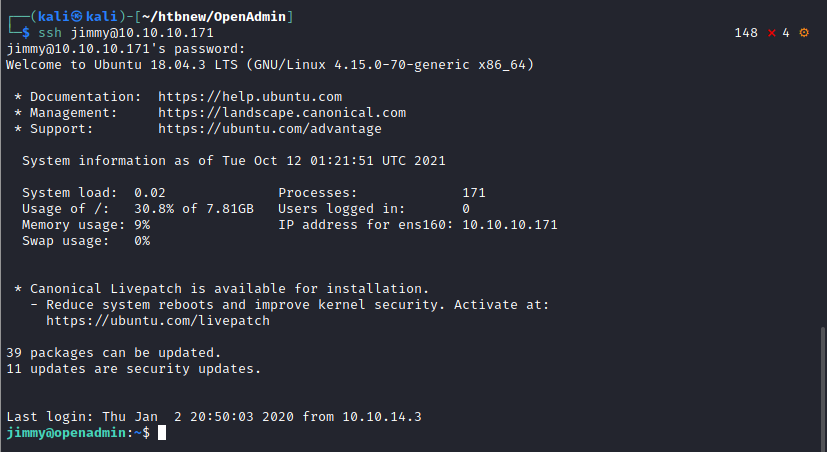
\includegraphics[width=0.8\textwidth]{images/openadmin/10-sshjimmy.png}
	\caption{Conexión SSH a jimmy}
\end{figure}

Revisando el contenido de /home/jimmy observamos que no se encuentra el archivo con la flag del usuario por lo que sugiere que el usuario que debemos tener control es joanna.
Utilizando la herramienta LinEnum, el cual es un script que realiza enumeración y chequeos para el escalamiento de privilegios. (https://raw.githubusercontent.com/rebootuser/LinEnum/master/LinEnum.sh) Vemos que tiene coneciones TCP. Sospechamos que debe ser el contenido que se encuentra en /var/www/internal.
\begin{figure}[H]
	\center
	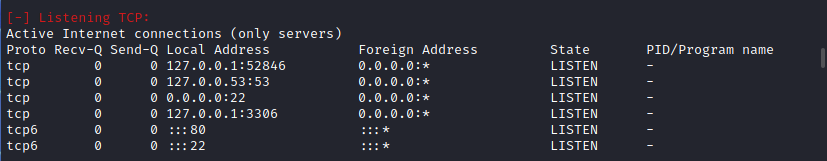
\includegraphics[width=0.8\textwidth]{images/openadmin/11-tcp.png}
	\caption{Conexiones TCP}
\end{figure}

\subsubsection{Obtención de Acceso como usuario joanna}

Realizamos curl http://127.0.0.1:52846 para ver el contenido de la página web y comprobamos que es el mismo que se encuentra en index.php, una página de login. Inspeccionando el archivo nos damos cuenta que está hardcodeado una contraseña hasheada con el algoritmo SHA512. 
\begin{figure}[H]
	\center
	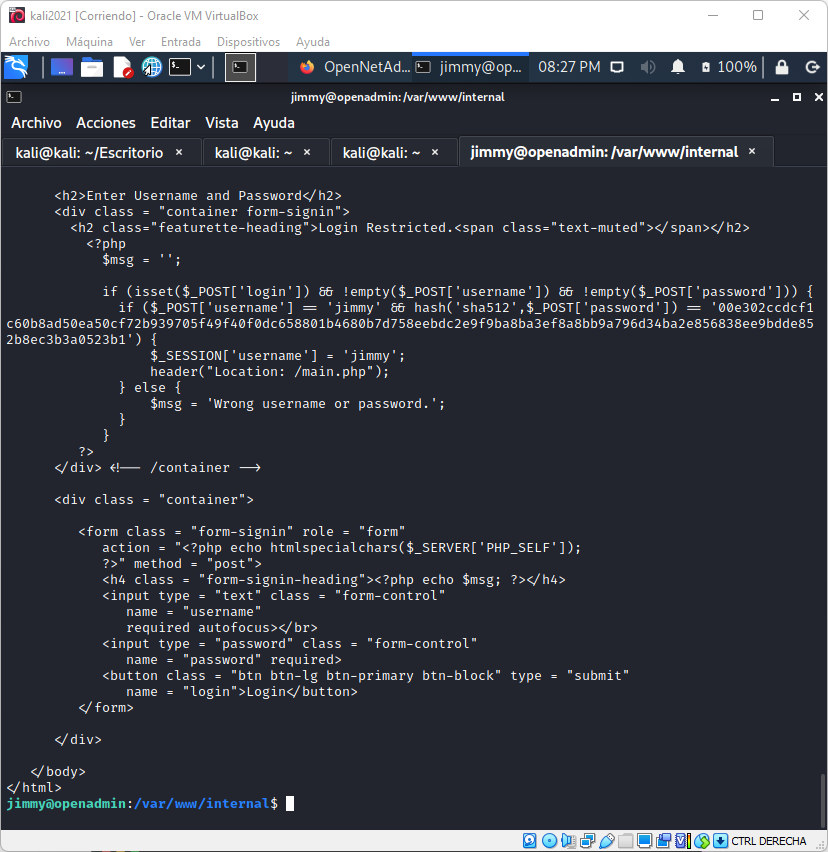
\includegraphics[width=0.8\textwidth]{images/openadmin/12-indexphp.png}
	\caption{index.php}
\end{figure}

Utilizando crackstation o John the Ripper se puede crackear el hash y el resultado es `Revealed'. El cual podemos utilizarlo para logearnos. Una vez logeado nos muestra una llave SSH encriptada que podría ser utilizada para alguna conexión ssh el cual podría ser la de joanna. Esto lo comprobamos al revisar el archivo main.php que ejecuta el comando `cat /home/joanna/.ssh/id\_rsa'.
\begin{figure}[H]
	\center
	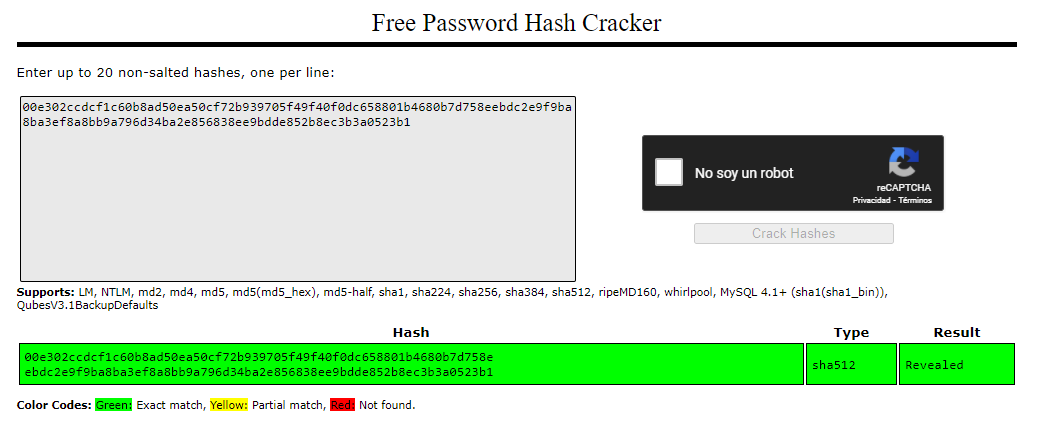
\includegraphics[width=0.8\textwidth]{images/openadmin/13-crackstation.png}
	\caption{Crackeo del hash}
\end{figure}

\begin{figure}[H]
	\center
	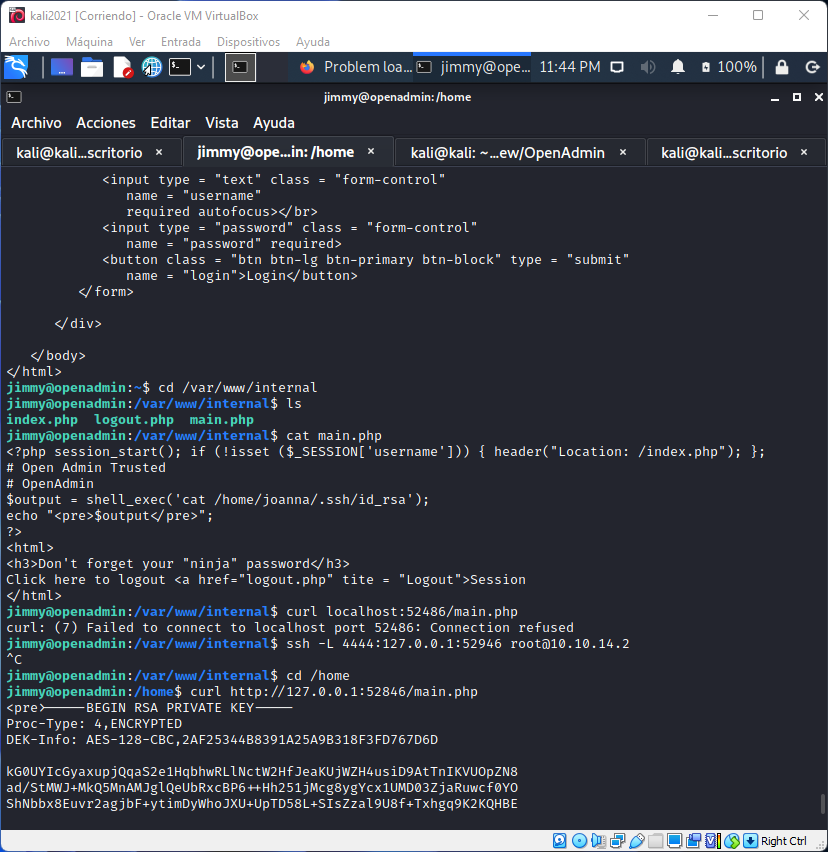
\includegraphics[width=0.8\textwidth]{images/openadmin/14-mainphp.png}
	\caption{index.php}
\end{figure}

\begin{figure}[H]
	\center
	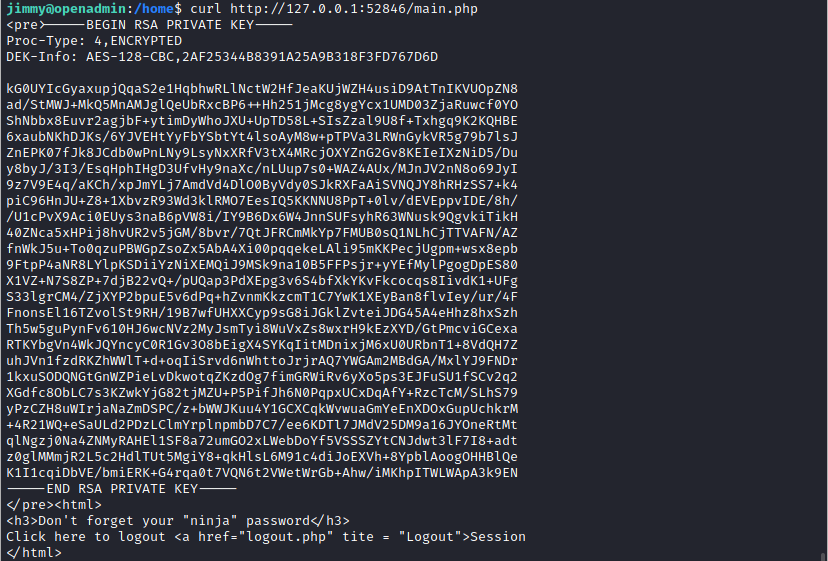
\includegraphics[width=0.8\textwidth]{images/openadmin/15-joannarsa.png}
	\caption{Llave RSA de joanna}
\end{figure}

Utilizando ssh2john y john logramos encontrar que la contraseña del hash es: bloodninjas
Como ya tenemos la contraseña y la llave RSA podemos establecer una conexión SSH a la máquina con el usuario joanna.
\begin{figure}[H]
	\center
	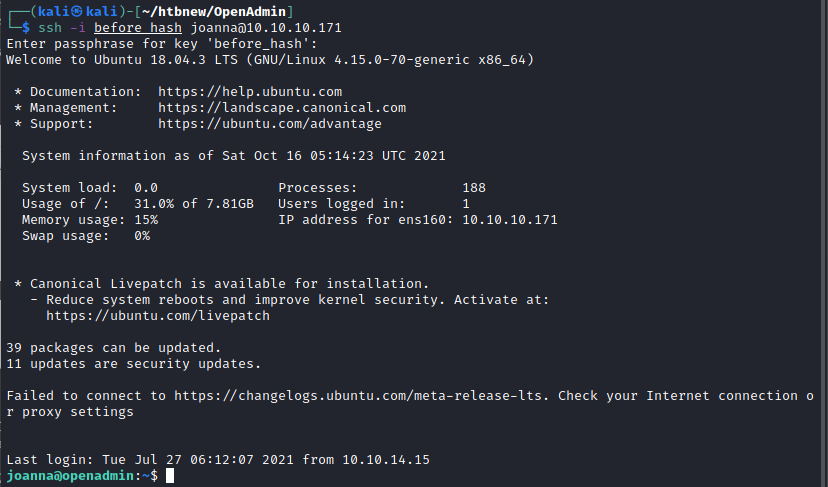
\includegraphics[width=0.8\textwidth]{images/openadmin/16-sshjoanna.png}
	\caption{Conexión SSH con el usuario joanna}
\end{figure}

Aunque como tenemos acceso a los archivos de la página web podemos simplemente agregar una reverse Shell y de esta forma obtener acceso a la máquina como el usuario joanna. Y esta vez vemos que tiene el archivo user.txt que es la flag del user
\begin{figure}[H]
	\center
	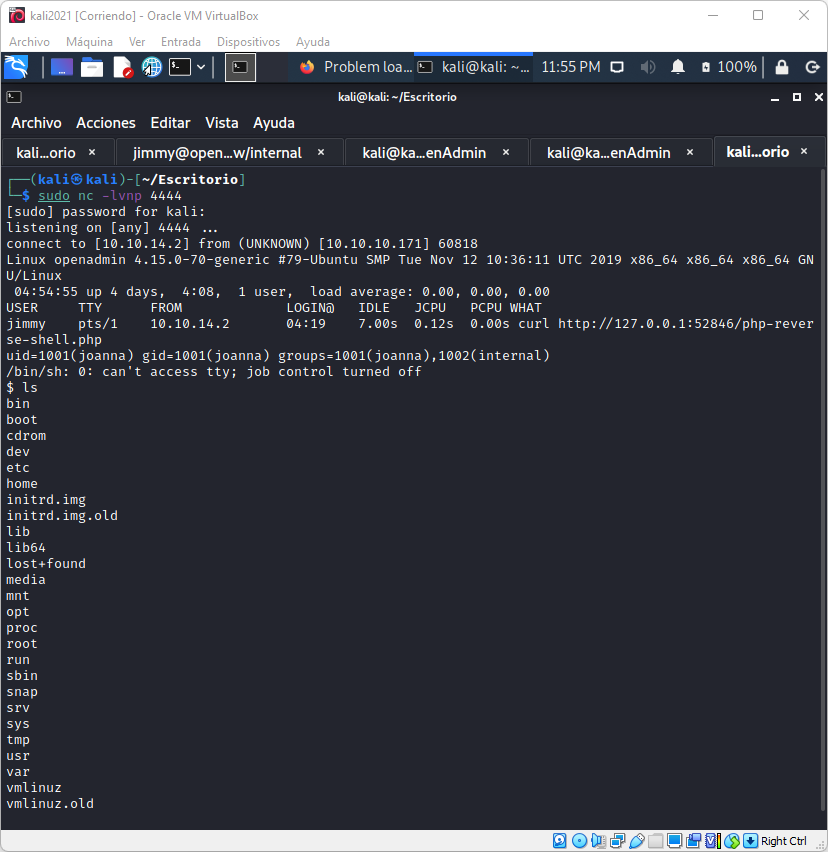
\includegraphics[width=0.8\textwidth]{images/openadmin/17-alternativa.png}
	\caption{main.php}
\end{figure}

\begin{figure}[H]
	\center
	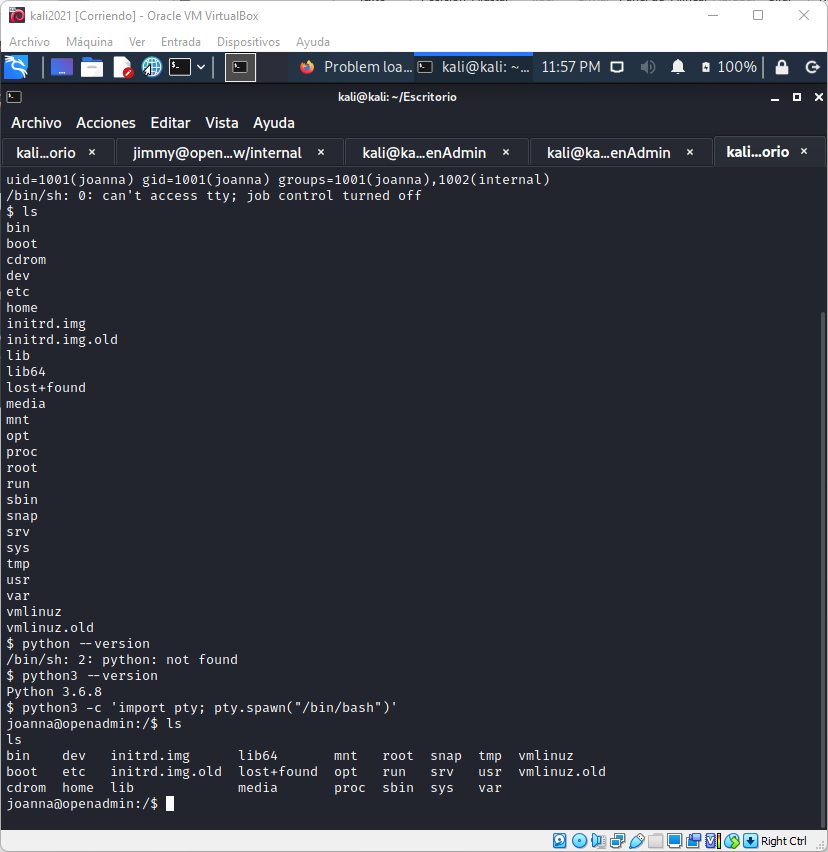
\includegraphics[width=0.8\textwidth]{images/openadmin/17-alternativa2.png}
	\caption{Mejora de la shell con Python pty}
\end{figure}

\begin{figure}[H]
	\center
	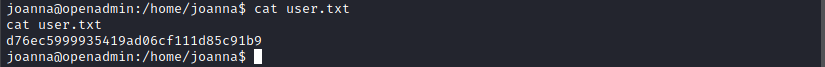
\includegraphics[width=0.8\textwidth]{images/openadmin/17-alternativa3.png}
	\caption{Flag del usuario}
\end{figure}

\subsection{Escalamiento de privilegios}

Una vez obtenido el acceso como joanna procederemos a revisar qué comandos podemos ejecutar como root.
\begin{figure}[H]
	\center
	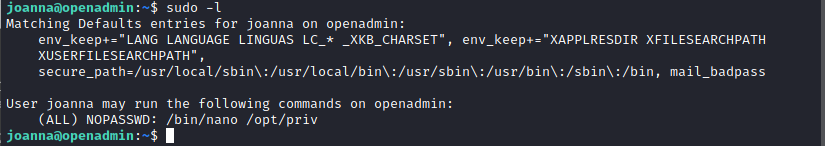
\includegraphics[width=0.8\textwidth]{images/openadmin/18-sudol.png}
	\caption{Comandos que puede ejecutar como root}
\end{figure}

Observamos que podemos ejecutar /bin/nano /opt/priv. Revisando GTFOBins, encontramos que podemos utilizar los siguientes comandos para generar un Shell de sistema interactivo mediante nano.
\begin{figure}[H]
	\center
	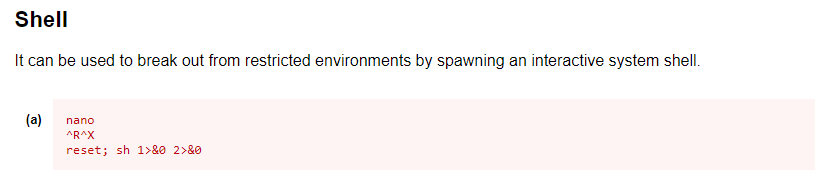
\includegraphics[width=0.8\textwidth]{images/openadmin/19-gtfobins.png}
	\caption{Exploit mediante sudo nano}
\end{figure}

Y de esta forma logramos obtener la flag del usuario root.
\begin{figure}[H]
	\center
	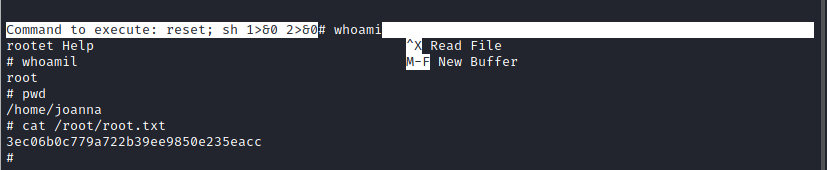
\includegraphics[width=0.8\textwidth]{images/openadmin/20-privilegio.png}
	\caption{Obtención del flag root}
\end{figure}

\subsection{Post Explotación}

Utilizamos perl para lograr una Shell reversa en nuestra máquina ya que es limitado y difícil de manejar en nano.
La Shell que obtenemos mediante la vulnerabilidad de sudo nano es simple por lo que es limitado y difícil de manejar. Por lo tanto, mediante una reverse Shell vamos a obtener la conexión en nuestra máquina configurando el puerto en escucha con NetCat. En este caso utilizaremos la reverse Shell de Perl.
\begin{figure}[H]
	\center
	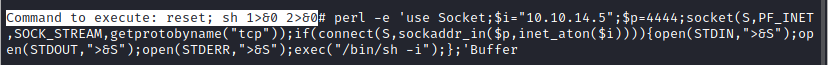
\includegraphics[width=0.8\textwidth]{images/openadmin/21-reverseshellperl.png}
	\caption{Código de la reverse shell con Perl}
\end{figure}

Una vez obtenida la Shell, podemos utilizar Python para mejorar la Shell a una completamente interactiva.
\begin{figure}[H]
	\center
	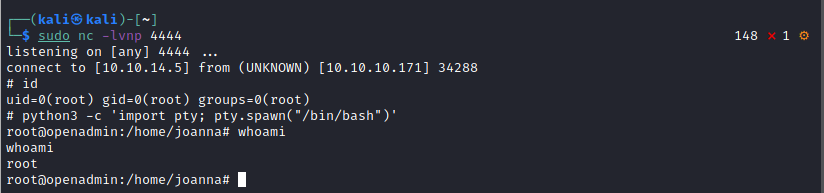
\includegraphics[width=0.8\textwidth]{images/openadmin/22-conexionreverse}
	\caption{Mejora de la shell con python}
\end{figure}

Procederemos a borrar nuestras huellas, limpiando los logs el cual podremos hacerlo manualmente o un script como por ejemplo “Cover my ass tool” (https://github.com/sundowndev/covermyass) que nos facilita la limpieza. Principalmente el log que buscamos limpiar es el auth.log el cual contiene los registros de todas las actividades que implican un proceso de autenticación.
\begin{figure}[H]
	\center
	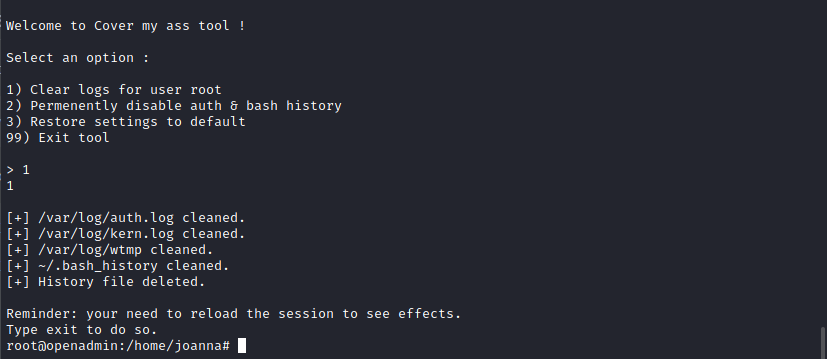
\includegraphics[width=0.8\textwidth]{images/openadmin/23-covermyass}
	\caption{Limpieza de logs con covermyass}
\end{figure}

\subsection{Hardening}
\begin{itemize}
	\item Cambiar los permisos para que solo los usuarios permitidos puedan leer los archivos de configuración.
	\item Evitar hardcodear las contraseñas para el login y utilizar una base de datos para almacenar las credenciales.
	\item Remover de sudoers la capacidad de utilizar ese comando con permisos de root si no es necesario.
\end{itemize}

\clearpage
% ----------------------------REMOTE-----------------------------------
\section{Remote}
\subsection{Reconocimiento}
Lo primero a hacer en este caso es un escaneo de nmap, para encontrar algunos puertos abiertos y servicios corriendo, en este caso se encontraron los puertos 21, 80 y 445 abiertos principalmente.

\begin{figure}[h]
	\center
	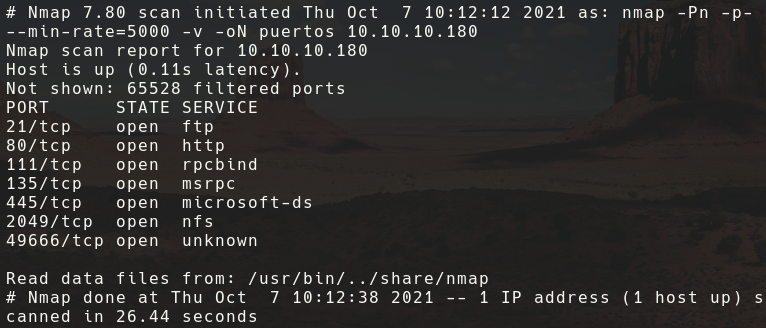
\includegraphics[width=0.8\textwidth]{images/remote/nmap_remote.png}
	\caption{nmap remote}
\end{figure}
 
\subsection{Escaneo de Vulnerabilidades}

Como primer escaneo de vulnerabilidades se intenta con el mismo nmap, con la opción "--script vuln", esto probará as vulnerabilidades más comunes en el server.

\begin{figure}[h]
	\center
	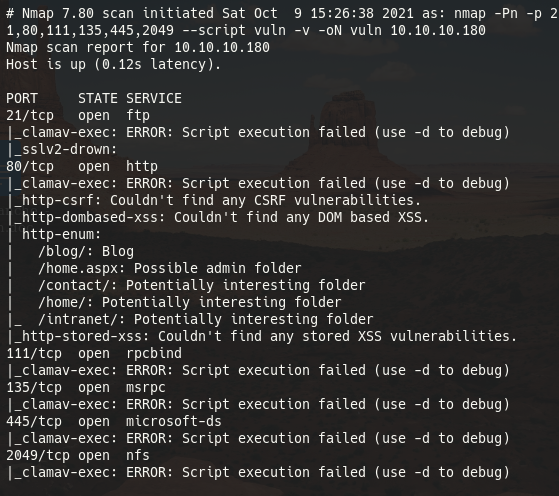
\includegraphics[width=0.7\textwidth]{images/remote/nmap_vuln.png}
	\caption{vulnerabilidades por nmap}
\end{figure}
\subsection{Enumeración}

Luego de ver los puertos, nmap no nos bota una vulnerabilidad por FTP, pero de todos modos nunca está de más probar si encontramos algo, sin embargo en esta ocasión no encontramos nada relevante.
\begin{figure}[h!]
	\center 
	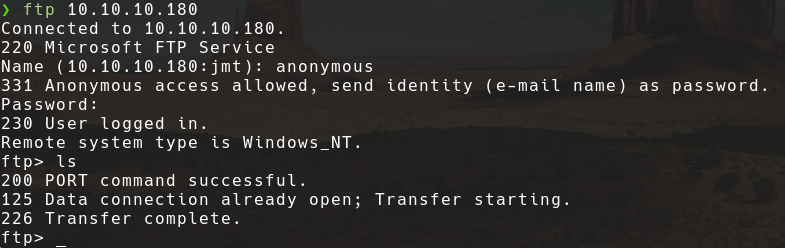
\includegraphics[width=\textwidth]{images/remote/ftp.png}
	\caption{logueo anónimo por FTP}
\end{figure}

Intentamos luego con la página ubicada en el puerto 80, a ver si encontramos algo, y efectivamente encontramos una página que tiene diferentes apartados para revisar, buscamos info en los cuadros y en toda la página pero es solo texto generado de relleno, así que no hay información relevante en estas páginas para diccionarios.
\begin{figure}[h!]
	\center 
	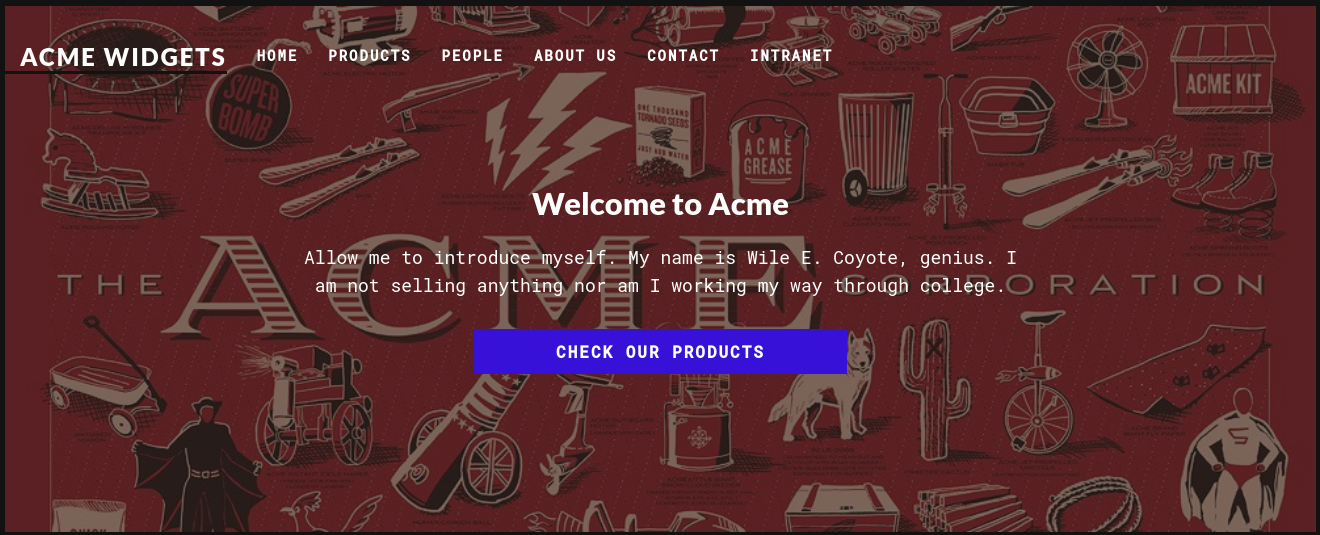
\includegraphics[width=\textwidth]{images/remote/index_pagina.png}
	\caption{logueo anónimo por FTP}
\end{figure}

\clearpage

Entre todas las páginas encontramos un apartado de login, está en el mismo servidor así que se ve bastante interesante junto a que el framework es de umbraco según el wappalizer.
\begin{figure}[h!]
	\center 
	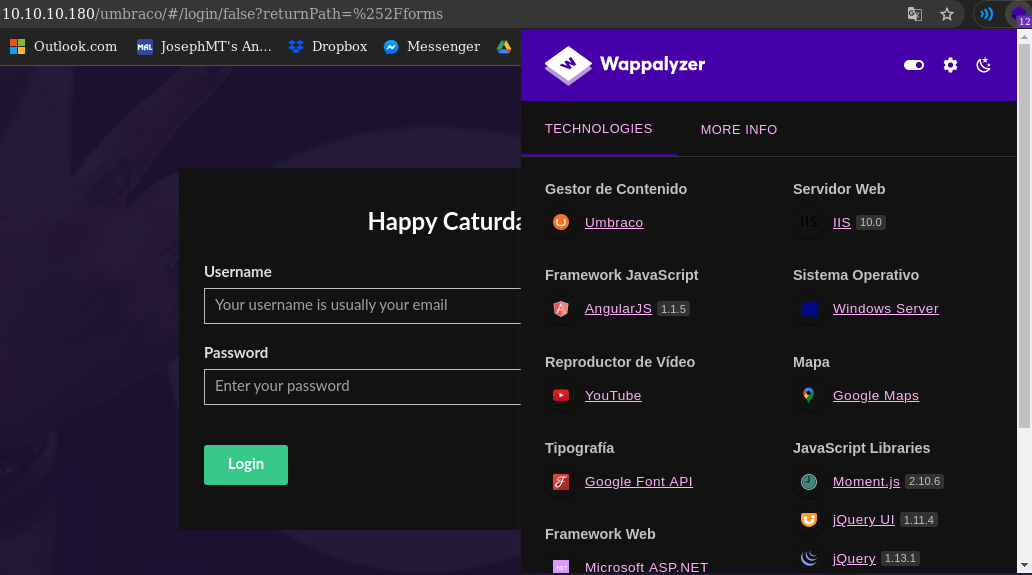
\includegraphics[width=0.9\textwidth]{images/remote/wappalizer.png}
	\caption{Resultados de wappalizer}
\end{figure}

Intentamos un escaneo con dirb para escanear los posibles directorios ocultos, donde se encontraron muchos directorios que de forma normal hubieran sido localizados y otros que hacen referencia a redirecciones, algunos que mostraron un error de configuración pero no grave.
\begin{figure}[h!]
	\center 
	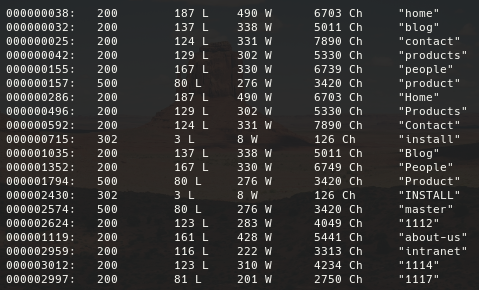
\includegraphics[width=0.9\textwidth]{images/remote/dirb.png}
	\caption{Escaneo con la herramienta dirb}
\end{figure}

\clearpage

Luego para tratar de buscar por los archivos compartidos se usa el comando llamado showmonts, que viene en la herramienta nfs-common.
\begin{figure}[h]
	\center 
	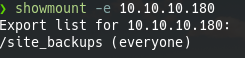
\includegraphics[width=0.6\textwidth]{images/remote/nfs.png}
	\caption{Obtención del backup}
\end{figure}

Luego creando una carpeta para guardar el contenido extraído con el comando "mount -t nfs 10.10.10.180:/site\_backups".
\\ una vez copiado esto tenemos carpetas interesantes, nuestro objetivo parecen ser credenciales de la base de datos para por medio de esas acceder al servidor original, entonces primero buscamos un poco.
\begin{figure}[h]
	\center 
	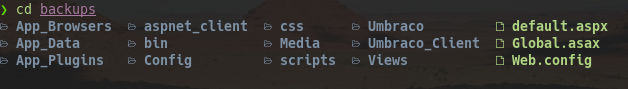
\includegraphics[width=\textwidth]{images/remote/backup.png}
	\caption{Revisado del backup}
\end{figure}
Entonces encontramos una password en hash dentro de "App\_Data/Umbraco.sdf"
La obtuvimos mediante el comando strings probando en diferentes archivos de configuración grepeando pass, luego de encontrarla en esta ruta vimos que grepeando pass no nos daba mucha información adicional al correo de login, así que probamos otro filtro.
\begin{figure}[h]
	\center 
	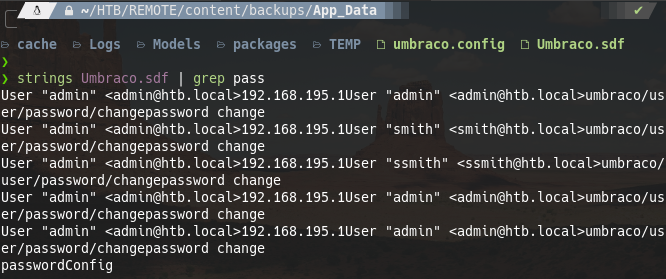
\includegraphics[width=\textwidth]{images/remote/strings_pass.png}
	\caption{Encontrando el fichero con la contraseña}
\end{figure}

\clearpage

Entonces probando el filtro "admin" en base a los resultados anteriors, y encontramos un hash, el cual mediante hash-identifier pudimos comprobar su naturaleza SHA1.
\begin{figure}[h]
	\center 
	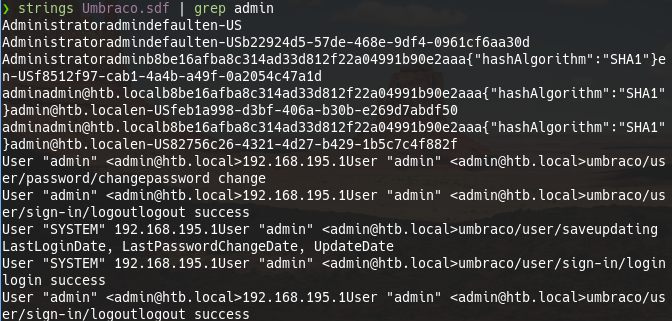
\includegraphics[width=\textwidth]{images/remote/strings_admin.png}
	\caption{Encontrando la contraseña cifrada}
\end{figure}

Ahora posteriormente lo que sigue es intentar el crackeo de esta contraseña cifrada en SHA1, para nuestra suerte este tipo de cifrado es completamente obsoleto al poseer posiblidad de colisiones en su algoritmo.
Por lo cual en diferentes sitios online se pueden encontrar formas de crackear la contraseña, y el resultado es la obtención de la contraseña "baconandcheese".
\begin{figure}[h!]
	\center 
	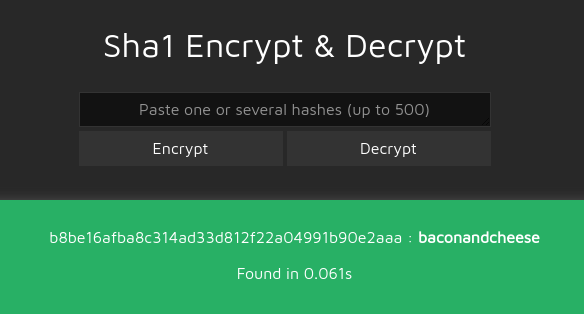
\includegraphics[width=\textwidth]{images/remote/sha1.png}
	\caption{Encontrando la contraseña en texto claro}
\end{figure}

\clearpage

Probando ya tenemos acceso a la página de administrador dentro de la página, donde se permite el subido de imágenes, lo cual nos hace dar una idea de una posible inyección o ejecución remota de comandos, para lo cual primero buscaremos si existe algún exploit que aproveche esta vulerabilidad en github.
\begin{figure}[h]
	\center 
	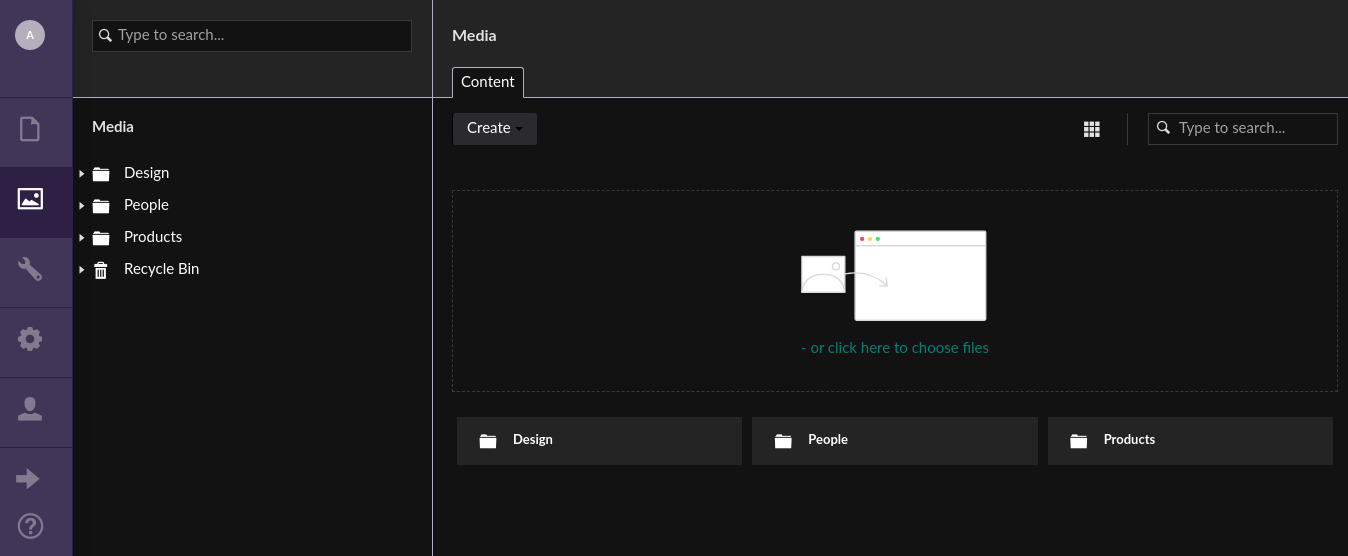
\includegraphics[width=\textwidth]{images/remote/admin-panel.png}
	\caption{Entrando al admin de Umbraco}
\end{figure}


\subsection{Explotación}
\subsubsection{Obtención de Acceso como usuario}
Entonces comenzamos con la búsqueda del script en github, para lo cual nos encontramos el siguiente. \textbf{\href{https://github.com/noraj/Umbraco-RCE}{https://github.com/noraj/Umbraco-RCE}}
Descargando el exploit y ejecutándolo obtenemos una ejecución remota de comandos mediante powershell.
\begin{figure}[h]
	\center 
	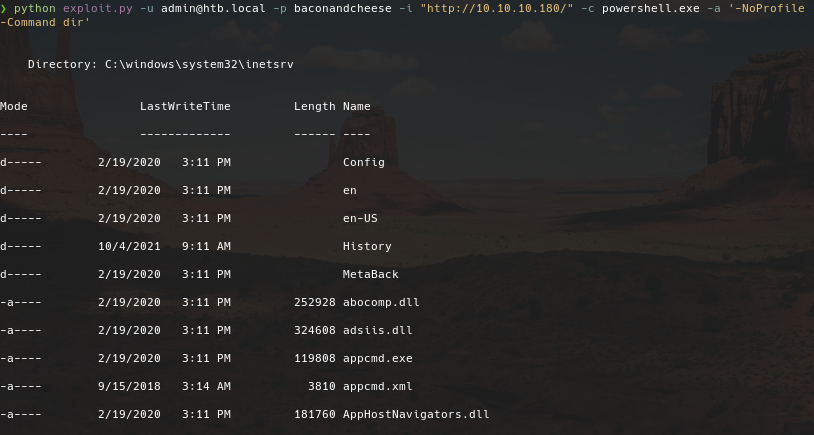
\includegraphics[width=\textwidth]{images/remote/script-1.png}
	\caption{Probando Ejecución Remota de Comandos}
\end{figure}

\clearpage

Una vez con esto tenemos que encontrar la forma de abrir una reverse shell para trabajar cómodos y explorar el sistema, entonces usarmos primero:
\begin{enumerate}
	\item Un Comando que permita la reverse shell que evite que crashee la terminal. Este lo obtenemos de diferentes payloads de \textbf{\href{https://github.com/swisskyrepo/PayloadsAllTheThings/blob/master/Methodology\%20and\%20Resources/Reverse\%20Shell\%20Cheatsheet.md\#powershell}{https://github.com/swisskyrepo/PayloadsAllTheThings.}}
	\begin{figure}[h]
		\center
		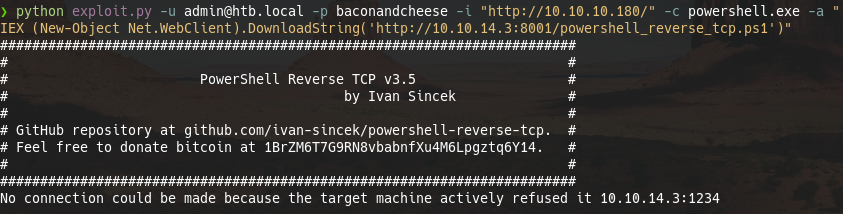
\includegraphics[width=0.9\textwidth]{images/remote/exploit.png}
		\caption{Comando del exploit}
	\end{figure}
	\item Levantamos un servidor en python3 para poder subir el payload al sistema y crear el backdoor.
	\begin{figure}[h]
		\center
		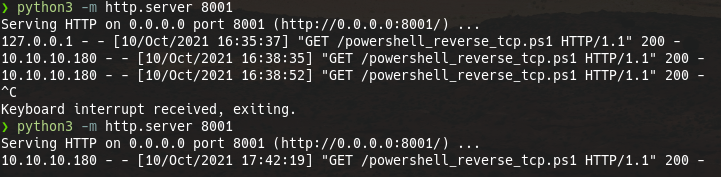
\includegraphics[width=0.9\textwidth]{images/remote/server-python.png}
		\caption{Server de Python3 en escucha}
	\end{figure}
	\item Un payload para establecer la conexión, este lo obtenemos de \textbf{\href{https://github.com/ivan-sincek/powershell-reverse-tcp/blob/master/src/powershell_bind_tcp.ps1}{https://github.com/ivan-sincek/powershell-reverse-tcp.}}.
	\begin{figure}[h]
		\center
		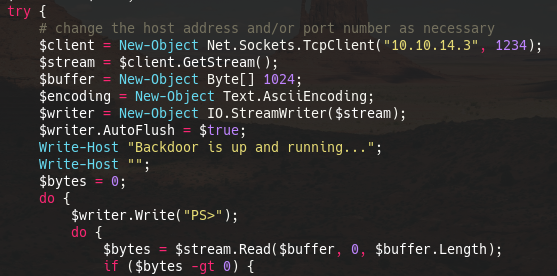
\includegraphics[width=0.9\textwidth]{images/remote/payload.png}
		\caption{Imagen del payload modificado con nuestra dirección}
	\end{figure}
\clearpage
	\item Tener escuchando con netcat un puerto para establecer la conexión por el payload.
	\begin{figure}[h!]
		\center
		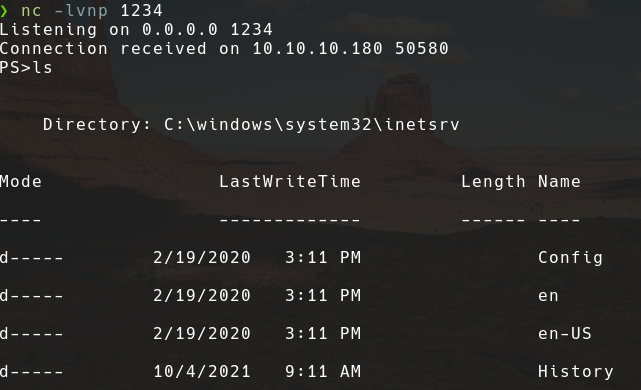
\includegraphics[width=0.9\textwidth]{images/remote/netcat.png}
		\caption{Estableciendo contacto con el netcat}
	\end{figure}
	\item Por último solo quedaría acceder a la carpeta del usuario y abrir el user.txt 
	\begin{figure}[h!]
		\center
		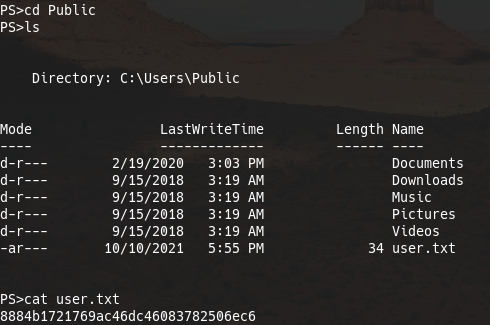
\includegraphics[width=0.9\textwidth]{images/remote/flag-usuario.png}
		\caption{Observando en texto claro la flag}
	\end{figure}

\end{enumerate}

\clearpage

\subsubsection{Escalamiento de Privilegios}
Para el escalamiento de privilegios lo primero que hice fue fijarme en los permisos que tenía con mi usuario actual, esto se puede hacer mediante el comando "whoami /priv".
\begin{figure}[h]
	\center
	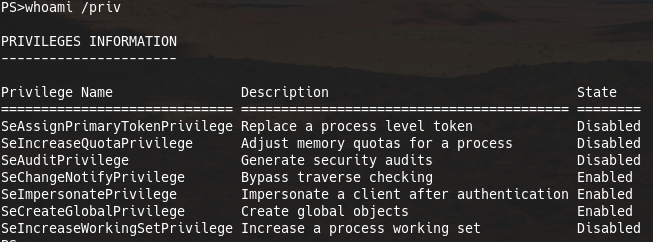
\includegraphics[width=\textwidth]{images/remote/privilegios.png}
	\caption{Verificando Privilegios}
\end{figure}
Luego de esto, había que averiguar la versión del sistema para poder empezar a buscar algún exploit relacionado a los permisos habilitados.
\begin{figure}[h]
	\center
	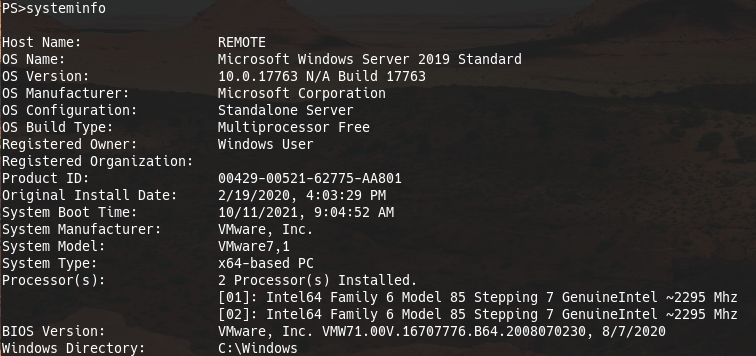
\includegraphics[width=\textwidth]{images/remote/systeminfo.png}
	\caption{Información del Sistema}
\end{figure}

\clearpage

Entonces encontramos un github que hablaba sobre el abuso del permiso \textbf{SeImpersonatePrivilege} en servidores 2016-2019, entonces mediante el script encontrado en : \\ \textbf{\href{https://github.com/itm4n/PrintSpoofer/tree/v1.0}{https://github.com/itm4n/PrintSpoofer/tree/v1.0}} 
\\ Luego de pasar el script a la máquina víctima mediante el uso de un servidor local en python3 y el comando en powershell invoke-webrequest que sirve a modo de wget para obtener una descarga de otro servidor.
el script llamado exploit.exe y el netcat llamado nc.exe son necesarios para poder levantar la reverse shell con permisos elevados.

\begin{figure}[h]
	\center
	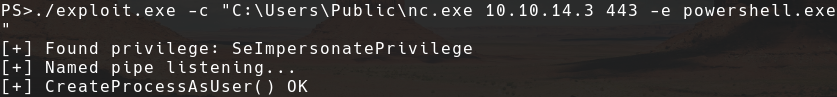
\includegraphics[width=\textwidth]{images/remote/fallo-exploit.png}
	\caption{Ejecutando el script de elevación.}
\end{figure}
Aparentemente funciona pero luego no detecta nada en el puerto de escucha, se hizo una corroboración por md5 a ver si el archivo era exactamente el mismo, pero debido a ciertas circunstancias esta forma no se dejó.
\begin{figure}[h]
	\center
	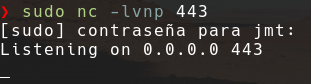
\includegraphics[width=0.4\textwidth]{images/remote/fallo-escucha.png}
	\caption{Fallo en la escucha}
\end{figure}
Entonces al fallar esta forma empecé a ver los procesos del sistema a ver si había alguna pista sobre cómo escalar privilegios, encontré todos los procesos no terminados del exploit que estaban corriendo en background.
y entonces encontré un proceso de TeamViewer7 corriendo.
\begin{figure}[h]
	\center
	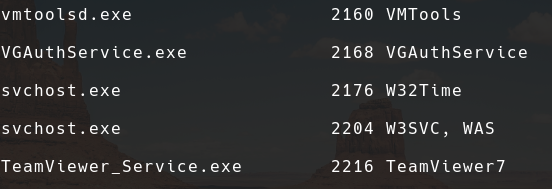
\includegraphics[width=0.7\textwidth]{images/remote/proceso-encontrado.png}
	\caption{Proceso de TeamViewer}
\end{figure}
Buscando un poco sobre algún exploit relacionado a la versión 7, encontré una forma de dumpear las claves de registro que se encuentran en ciertas rutas, un poco más de la documentación se encuentra en : 
\textbf{\href{https://whynotsecurity.com/blog/teamviewer/}{https://whynotsecurity.com/blog/teamviewer/}}

\clearpage

Entonces nos dirigimos a la ruta en cuestión para poder dumpear la clave de registro.
\begin{figure}[h]
	\center 
	\includegraphics[width=0.8\textwidth]{images/remote/confirmación-hash.png}
	\caption{Verificando llave disponible}
\end{figure}

Ya averiguamos de qué parámetro tenemos que buscar la llave, googleando un poco encontramos la ruta y es la siguiente, entonces solo tocaría dumpear.
\begin{figure}[h!]
	\center 
	\includegraphics[width=0.5\textwidth]{images/remote/dumpeo-hash.png}
	\caption{Dumpeando la clave}
\end{figure}

\clearpage

Ahora lo que sigue es crackear esta contraseña, según vimos en la vulnerabilidad usa un cifrado AES-128-CBC con la llave 0602000000a400005253413100040000, encontré un script que se usaba para dumpear las credenciales de este exploit específicamente y es el siguiente.
\begin{figure}[h]
	\center 
	\includegraphics[width=\textwidth]{images/remote/script-python-hash.png}
	\caption{Script de Python para decifrar la clave}
\end{figure}

Con esto obtuvimos la contraseña que era \textbf{!R3m0te!}, ya con esta clave obtenida podemos usar algún impacket para acceder a la máquina, en este caso usamos el psexec.py ubicando el github \textbf{\href{https://github.com/SecureAuthCorp/impacket/blob/master/examples/psexec.py}{https://github.com/SecureAuthCorp/}}.
\begin{figure}[h]
	\center 
	\includegraphics[width=\textwidth]{images/remote/exito-administrator.png}
	\caption{entrando como NT Authority System}
\end{figure}

Con esto ya podríamos obtener la bandera root en C:\textbackslash Users\textbackslash Administrator\textbackslash Desktop\textbackslash root.txt.
Y así finalizaría el acceso completo a la máquina Remote, con los máximos privilegios se puede hacer de todo, así que con esto en mente lo que sigue ahora es la parte de post explotación, en la cual principalmente se hará el hardening de las vulnerabilidades para que no haya problemas críticos en la seguridad.
\clearpage

\subsection{Hardening}

\subsubsection{Umbraco}

Para evitar el ingreso por el vector de umbraco se requiere una actualización, pero debido a que pasar de Umbraco 7 al 8 o 9 no es tan sencillo, gracias a la incompatibilidad de código que hay entre versiones, la única solución que quedaría sería netamente pasar el contenido de forma manual de una versión a otra.
Esta es la solución oficial que nos dan en la documentación de Umbraco, sin embargo esta versión es completamente obsoleta así que solo quedaría hacer la migración manual como sugieren.
De hecho gracias a la versión que se tiene en el servidor, que es la 7.12.4, no tiene forma de migrar.
\begin{figure}[h]
	\center 
	\includegraphics[width=0.3\textwidth]{images/remote/umbraco-version.png}
	\caption{Solución Oficial de Umbraco}
\end{figure}
\\ Entonces la única solución sería instalar una nueva versión de Umbraco 9 y configurar el servidor desde esa base.

\subsubsection{Permisos Powershell}

También se tuvo un problema con los permisos o privilegios que tenía el usuario con el que se escaló privilegios, debido a la versión 2019 de servidor que se usaban era necesario verificar que el permiso \textbf{SeImpersonatePrivilege}-
Para lo cual se tiene que deshabilitar mediante un script referenciado en 


\begin{lstlisting}
	function Add-ServiceLogonRight([string] $Username) {
		Write-Host "Enable ServiceLogonRight for $Username"
	
		$tmp = New-TemporaryFile
		secedit /export /cfg "$tmp.inf" | Out-Null
		(gc -Encoding ascii "$tmp.inf") -replace '^SeServiceLogonRight .+
		', " `$0,$Username" | sc -Encoding ascii "$tmp.inf"
		secedit /import /cfg "$tmp.inf" /db "$tmp.sdb" | Out-Null
		secedit /configure /db "$tmp.sdb" /cfg "$tmp.inf" | Out-Null
		rm $tmp* -ea 0
	}
\end{lstlisting}	

Con esto ya evitaría que se pueda escalar privilegios mediante el exploit en Windows Server 2019.

\subsubsection{TeamViewer7}

Para instalar esto se necesitaría o eliminar el proceso o actualizar la versión a la más nueva, pero desde cmd o powershell no se puede actualizar de forma sencilla los programas debido a la forma en la que están hechos y el funcionamiento de la terminal en windows.
De todos modos se podría actualizar luego de instalar un programa llamado winget ubicado en \textbf{\href{https://github.com/microsoft/winget-cli/releases}{https://github.com/microsoft/winget-cli/releases}}


\clearpage
% ----------------------------FUSE-----------------------------------
\section{Fuse}
\subsection{Reconocimiento}

Hack The Box proporcionó los datos del servidor el cual deberá ser auditado, el cual tiene las características descritas en la Figura \ref{fuse_logo}

\begin{figure}[h]
	\center
	\includegraphics[width=0.6\textwidth]{images/fuse/fuse_logo.png}
	\caption{Reconociendo puertos abiertos.}
	\label{fuse_logo}
\end{figure}

\subsection{Escaneo de Vulnerabilidades}

Realizamos un escaneo más profundo al incluir algunas opciones adicionales que nos brinden mayor detalle del servidor objetivo. En este caso, usamos algunas opciones como escanear todos los puertos y el escaneo de versiones de los servicios que están corriendo en cada puerto.

\begin{figure}[h]
	\center
	\includegraphics[width=0.8\textwidth]{images/fuse/services.png}
	\caption{Reconociendo puertos abiertos.}
\end{figure}

Se identifican servicios importantes tales como:
\begin{itemize}
	\item DC: Fabricorp.local
	\item Servicio Web: Puerto 80
	\item Servicio Samba: Puerto 445
	\item Servicio RPC: Puerto 135
	\item Servicio RDP: Puerto 5985
\end{itemize}

\clearpage

\subsection{Enumeración}

Partimos revisando el servicio web, para lo cual ingresamos desde un navegador a la IP que tenemos, notando que se está realizando una redirección a una ruta específica, la cual no está registrada en nuestro equipo.
\begin{figure}[h]
	\center
	\includegraphics[width=0.8\textwidth]{images/fuse/image2.png}
	\caption{Primer intento de acceso al servicio Web de Fuse}
\end{figure}

Para poder acceder sin problemas, entonces agregamos dicha ruta y la IP en el archivo /etc/hosts, como se muestra en la Figura \ref{fuse_hosts}

\begin{figure}[h]
	\center
	\includegraphics[width=0.8\textwidth]{images/fuse/image3.png}
	\caption{Contenido del archivo hosts.}
	\label{fuse_hosts}
\end{figure}

Ahora, al probar nuevamente, podemos confirmar que ya se tiene acceso al sitio web, y con ello descubrimos que en dicho sitio web está alojado un servicio de logs de impresión, así como se muestra en la Figura \ref{fuse_webpage}.

\begin{figure}[h]
	\center
	\includegraphics[width=0.7\textwidth]{images/fuse/image4.png}
	\caption{Sitio web de Fuse.}
	\label{fuse_webpage}
\end{figure}

\clearpage

Explorando el sitio web, se notó que entre los logs que se almacenan se tiene al menos como información los usuarios, el nombre del archivo que imprime y la impresora, y todo esto para 3 fechas.

\begin{figure}[h]
	\center
	\includegraphics[width=0.8\textwidth]{images/fuse/image5.png}
	\caption{Fechas registradas en PaperCut.}
\end{figure}
\vfill
\begin{figure}[h]
	\center
	\includegraphics[width=0.8\textwidth]{images/fuse/image6.png}
	\caption{Logs de impresión almacenados.}
\end{figure}

De dicha información, la que notamos que nos servirá más adelante es el dato del USER, así que generamos un archivo users.txt para guardarlos. Los usuarios encontrados fueron: \textbf{pmerton, benielson, tlavel, sthompson, administrator y bhult.}

Así mismo, a partir de los archivos que están imprimiendo, generamos una lista de palabras para encontrar si alguna ha sido usada como contraseña.

\vfill
\vfill

\subsection{Explotación}

Procedemos de esta forma a utilizar Crackmapexec, el cual nos permitirá probar en conjunto los usuarios y las potenciales claves.

\begin{figure}[h]
	\center
	\includegraphics[width=0.8\textwidth]{images/fuse/image7.png}
	\caption{...}
\end{figure}

Vemos un comportamiento diferente al tratar de usar como contraseña “Fabricorp01”. Aunque debido a que no se completa la ejecución para todos los usuarios, procedemos a realizar la ejecución manual para todos los usuarios capturados previamente.

\clearpage 


\begin{figure}[h]
	\center
	\includegraphics[width=0.8\textwidth]{images/fuse/image8.png}
	\caption{Usuarios identificados con contraseña vencida.}
\end{figure}
\vfill
A partir de esto, los usuarios que tienen un comportamiento similar es \textbf{tlavel, bhult y bnielson}. Si revisamos lo que se indica, podemos saber que dichos usuarios tienen la clave “Fabricorp01” pero está vencida, probablemente por una política de cambio de contraseñas, así que la siguiente actividad sería cambiar dicha clave por una de nuestra conveniencia.
Para dicho cambio usamos smbpasswd e ingresamos una contraseña cualquiera. (En este caso “Prueba123”).

\begin{figure}[h]
	\center
	\includegraphics[width=0.8\textwidth]{images/fuse/image9.png}
	\caption{Actualizando la clave de un usuario de Fuse.}
\end{figure}

\vfill
Habiendo cambiado las credenciales del usuario bnielson, el siguiente paso sería listar listar el contenido de lo que comparte dicho usuario, para lo cual nos apoyamos de la herramienta smbmap. 

\begin{figure}[h]
	\center
	\includegraphics[width=0.8\textwidth]{images/fuse/image10.png}
	\caption{Usando SMBMap para identificar directorios o equipos conectados.}
\end{figure}

\vfill
Un punto a tener en cuenta, es que, habiando realizado el cambio de contraseña del usuario bnielson, igualmente tras un intento de autenticación con dichas credenciales, como por ejemplo, el usar el smbmap o crackmapexec, notamos que cada vez se está reiniciando la contraseña, volviendo a ser la inicial la cual era “Fabricorp01”. Para un ataque más complejo, podría considerarse el desarrollo de una herramienta que automatice dicho cambio para realizar más pruebas, aunque en este caso no fue necesario. Lo descrito anteriormente puede ser notado en la Figura \ref{fail_fuse}


\clearpage


\begin{figure}
	\center
	\includegraphics[width=0.8\textwidth]{images/fuse/image11.png}
	\caption{Error de autenticación tras reinicio de clave automático.}
	\label{fail_fuse}
\end{figure}


Para mantener una sesión que nos permita mantenernos conectados sin tener que estar reiniciando la contraseña a cada momento, aprovechamos el servicio RPC usando la herramienta rpcconect.

\begin{figure}[h]
	\center
	\includegraphics[width=0.8\textwidth]{images/fuse/image12.png}
	\caption{Obteniendo el promt con RPCConnect}
\end{figure}

Ya conectados mediante RPC, procedemos a listar los usuarios registrados en el servidor con el comando enumdomusers, esto con la finalidad de incrementar la cantidad de usuarios potenciales que teníamos inicialmente y aumentar las probabilidades de encontrar una cuenta para ingresar.

\begin{figure}[h]
	\center
	\includegraphics[width=0.6\textwidth]{images/fuse/image13.png}
	\caption{Usuarios en Fuse listados mediante RPC}
\end{figure}

Debido a que se ha visto por el sitio web que hay impresoras instaladas, se provecha a explorar las que se encuentran conectadas con enumprinters y terminamos encontrando una contraseña dejada en la descripción para posiblemente los colaboradores de la organización.

\begin{figure}[H]
	\center
	\includegraphics[width=0.8\textwidth]{images/fuse/image14.png}
	\caption{Credenciales encontradas en la descripción de una impresora.}
\end{figure}

Con la nueva contraseña encontrada, procedemos a probar nuevamente con cada usuario que encontramos con rpc. En este caso usaremos Hydra. 
\clearpage
\begin{figure}[h]
	\center
	\includegraphics[width=0.8\textwidth]{images/fuse/image15.png}
	\caption{Claves confirmadas usando Hydra.}
\end{figure}

Ahora, con el objetivo de tener acceso a una consola interactiva aprovecharemos RDP, mediante la herramienta evil-WinRM, con el cual obtenemos una shell con la máquina.

\begin{figure}[h]
	\center
	\includegraphics[width=0.8\textwidth]{images/fuse/image16.png}
	\caption{Conexión exitosa con el servidor usando el usuario svc-print}
\end{figure}

Con ello obtuvimos el primer archivo importante que en esta máquina es user.txt.

\begin{figure}[h]
	\center
	\includegraphics[width=0.7\textwidth]{images/fuse/image17.png}
	\caption{Bandera de usuario encontrada.}
\end{figure}
\vfill
\textbf{Escalando privilegios}

Revisando recordamos la existencia de una de las vulnerabilidades más importantes encontradas últimamente, y es la de ZeroLogon, la cual permite obtener la totalidad de las credenciales en formato HASH. 
Para ejecutar dicha vulnerabilidad, aprovechamos el exploit elaborado por Risksense alojado en \href{https://github.com/risksense/zerologon}{GitHub} en el cual iniciamos ejecutando el script "set\_empty\_pw.py". 

\begin{figure}[H]
	\center
	\includegraphics[width=0.8\textwidth]{images/fuse/image18.png}
	\caption{Ejecución exitosa del exploit ZeroLogon}
\end{figure}

\clearpage
Tras la ejecución exitosa, procedemos a utilizar Impacket para obtener las credenciales.

\begin{figure}[h]
	\center
	\includegraphics[width=0.8\textwidth]{images/fuse/image19.png}
	\caption{Obteniendo credenciales con Impacket}
\end{figure}

Teniendo las credenciales de los usuarios, podemos usar la del administrador para poder conectarnos usando evil-WinRm.

\begin{figure}[h]
	\center
	\includegraphics[width=0.8\textwidth]{images/fuse/image20.png}
	\caption{Usando las credenciales para conectarse a la máquina vía RDP}
\end{figure}

Solo tendríamos que buscar el archivo valioso de este servidor, ubicado en la ubicación mostrada en la Figura \ref{get_root_fuse}

\begin{figure}[h]
	\center
	\includegraphics[width=0.8\textwidth]{images/fuse/image21.png}
	\caption{Bandera de usuario administrador obtenida.}
	\label{get_root_fuse}
\end{figure}
\clearpage


\subsection{Post Explotación}
\begin{itemize}
	\item Obteniendo SAM
	\begin{figure}[h]
		\center
		\includegraphics[width=0.8\textwidth]{images/fuse/sam.png}
		\caption{Obteniendo SAM.}

	\end{figure}
\end{itemize}

\subsection{Recomendaciones}
Para garantizar que el servidor no sea vulnerado, el equipo tiene las siguiente recomendaciones:
\begin{itemize}
	\item Instalar el parche KB4571723.
	
	Parche de seguridad importante lanzado por Microsoft para evitar la ejecución de exploits relacionados con la vulnerabilidad llamada ZeroLogon.
	\item Revisar política de contraseñas.
	
	Si bien la organización actualmente demuestra que está indicando periodos de validez a las contraseñas usadas, la práctica de reestablecerla a una versión anterior que no varía no se considera una práctica recomendada.

	\item Revisar que las contraseñas estén protegidas.
	Se recomienda usar un almacén de contraseñas para resguardarlas y evitar que terminen en recordatorios o puntos de fácil acceso para los atacantes.
\end{itemize}

\clearpage 

% ----------------------------MAGIC-----------------------------------
\section{MAGIC}
\subsection{Reconocimiento}
Lo primero a hacer en este caso es un escaneo de nmap, para encontrar algunos puertos abiertos y servicios corriendo, en este caso se encontraron los puertos 22 y 80. Esto nos da una idea de que todo se hace netamente por el acceso a página web del puerto 80, porque es muy raro encontrar vulnerabilidades del puerto 22.
\begin{figure}[h]
	\center 
	\includegraphics[width=\textwidth]{images/magic/nmap.png}
	\caption{Escaneo de Puertos con Nmap}
\end{figure}
Entonces vemos en el puerto 80 existe una página, decidimos escanear directorios mediante \textbf{Wfuzz} y al mismo tiempo vamos a observar la página.
\begin{figure}[h]
	\center 
	\includegraphics[width=\textwidth]{images/magic/wfuzz.png}
	\caption{Escaneo de Directorios con Wfuzz}
\end{figure}

\clearpage

Entonces entrando a la máquina podemos ver la página principal en el índice, vemos que hay muchas imágenes subidas y en caso de poder loguearnos nos dejaría subir unas cuantas más.
\begin{figure}[h!]
	\center 
	\includegraphics[width=\textwidth]{images/magic/index.png}
	\caption{Index de la página principal}
\end{figure}
Vemos aquí el apartado de login, este es algo simple y parece funcionar debido a que bota un error de contraseña incorrecta.
\begin{figure}[h!]
	\center 
	\includegraphics[width=\textwidth]{images/magic/login.png}
	\caption{Login de la página web}
\end{figure}

\clearpage

\subsection{Escaneo de Vulnerabilidades}

Llegó el momento de intentar encontrar vectores de ataque, con el mismo nmap dejamos corriendo un análisis de vulnerabilidades a los puertos 80 y 22 pero no encontró nada muy útil.
\begin{figure}[h!]
	\center 
	\includegraphics[width=\textwidth]{images/magic/nmap-vuln.png}
	\caption{Escaneo de Vulnerabilidades con nmap}
\end{figure}


\subsection{Explotación}
\subsubsection{Obtención de Acceso a la máquina}
Luego de esto fui al login y me di cuenta que el ataque de tipo Inyección SQL era muy sencillo, probando \textbf{' or 1=1 --}. Esta es la inyección más básica de toda la vida así que no hubo mucha complicación.

\begin{figure}[h!]
	\center 
	\includegraphics[width=\textwidth]{images/magic/login-existoso.png}
	\caption{Login existoso en la página web}
\end{figure}

\clearpage

Entonces vemos claramente una forma de subir una reverse shell con formato de imagen, probaremos primero subiendo una revershe shell en .php a ver si hay algún problema.

\begin{figure}[h!]
	\center 
	\includegraphics[width=\textwidth]{images/magic/fallo-subida-php.png}
	\caption{Fallo subiendo un php}
\end{figure}

Imaginaba que no iba a ser tan fácil así que abrí el burpsuite y traté de hacerlo pasar como imagen para luego borrar la extensión y ejecutarlo dentro del servidor.

\begin{figure}[h!]
	\center 
	\includegraphics[width=\textwidth]{images/magic/intento-burpsuit.png}
	\caption{Intento con Burpsuite}
\end{figure}

\clearpage

Luego intentando la subida también falló como se puede ver, este mensaje es diferente y nos hace sospechar que se tiene otro medio de verificar, por lo cual ahora intentaré con los bits mágicos de los archivos, los cuales podemos encontrar más información aquí: \\ 
\textbf{\href{https://en.wikipedia.org/wiki/List_of_file_signatures}{https://en.wikipedia.org/wiki/List\_of\_file\_signatures}}.

\begin{figure}[h!]
	\center 
	\includegraphics[width=\textwidth]{images/magic/fallo-burpsuite.png}
	\caption{Fallo con Burpsuite}
\end{figure}

Primero mostramos los bits mágicos que tenemos por defecto en nuestro archivo para verificar que es de un php convencional.

\begin{figure}[h!]
	\center 
	\includegraphics[width=\textwidth]{images/magic/muestra-bits.png}
	\caption{Bits previo al cambio}
\end{figure}

\clearpage

Entonces cambiamos los bits de inicio a los de un jpg, y luego editamos encima usando una revershe shell que está en el siguiente github: \textbf{\href{https://github.com/pentestmonkey/php-reverse-shell/blob/master/php-reverse-shell.php}{https://github.com/pentestmonkey/php-reverse-shell}}

\begin{figure}[h!]
	\center 
	\includegraphics[width=\textwidth]{images/magic/cambio-bits.png}
	\caption{Cambio de los bits del inicio}
\end{figure}

Luego de esto solo queda subir el archivo a ver esta vez no tenemos problemas, y efectivamente este se sube satisfactoriamente ya sin necesidad de editar nada en burpsuite.

\begin{figure}[h!]
	\center 
	\includegraphics[width=\textwidth]{images/magic/subida-exitosa.png}
	\caption{Subida de reverse shell exitosa}
\end{figure}

Ahora solo queda apuntar a la dirección donde se suben, felizmente para esto pudimos encontrar la ubicación con el fuzzeo anterior.


\begin{figure}[h!]
	\center 
	\includegraphics[width=\textwidth]{images/magic/apuntando-reverse1.png}
	\caption{Apuntando a nuestra reverse shell}
\end{figure}


\clearpage

Entonces si abrimos nuestro netcat escuchando por el puerto 1234, obtenemos respuesta y ganamos acceso al servidor.

\begin{figure}[h!]
	\center 
	\includegraphics[width=\textwidth]{images/magic/acceso-maquina.png}
	\caption{Acceso a la Máquina por netcat}
\end{figure}

Pero nos damos con la sorpresa de no poder ver la bandera de usuario.

\begin{figure}[h!]
	\center 
	\includegraphics[width=0.7\textwidth]{images/magic/fallo-lectura-flag.png}
	\caption{Fallo de lectura de la flag}
\end{figure}

\clearpage

\subsubsection{Obtención de Acceso como Usuario}

Ahora entonces lo que tenemos que hacer es un movimiento lateral para obtener un acceso a otro usuario.

Algo que nos impide ver los permisos sudo que tenemos es que no contamos con la contraseña, entonces exploramos un poco por el servidor pero encontramos un archivo curioso llamado \textbf{db.php5}.

\begin{figure}[h!]
	\center 
	\includegraphics[width=0.9\textwidth]{images/magic/credenciales-mysql.png}
	\caption{Credenciales del MySQL}
\end{figure}

Aquí encontramos las credenciales del MySQL, entonces intentamos conectarnos a este pero nos indica que no existe MySQL como comando, lo que significa que no existe el cliente con el cual nos podríamos conectar mediante consola, pero vemos en los procesos y sí está corriendo \textbf{mysqld}, entonces sabemos que el servicio está activo, esto nos deja con una opción, redirigir este servicio corriendo por un puerto hacia otro puerto.
Por lo cual haremos uso del programa \textbf{\href{https://github.com/jpillora/chisel}{chisel}}, este programa tendremos que correrlo tanto en la máquina server como cliente.
Levantamos un servidor con python por el puerto 8001 y lo descargamos con wget en la máquina remota.

\begin{figure}[h!]
	\center 
	\includegraphics[width=0.9\textwidth]{images/magic/descargar-chisel.png}
	\caption{Descarga de Chisel}
\end{figure}

\clearpage

Primero pondremos en escucha por el puerto 8000 a nuestra máquina.

\begin{figure}[h!]
	\center 
	\includegraphics[width=\textwidth]{images/magic/chisel-server.png}
	\caption{Chisel en escucha}
\end{figure}

Luego corremos el chisel en el servidor, la descarga la hicimos en /temp/jmt para que deje descargar.
\begin{figure}[h!]
	\center 
	\includegraphics[width=\textwidth]{images/magic/chisel-cliente.png}
	\caption{Chisel reenvíando flujo de puertos}
\end{figure}

Ya luego de haber hecho esto, podemos finalmente loguearnos al MySQL, con el comando respectivo y las credenciales obtenidas del \textbf{db.php5}.
\begin{figure}[h!]
	\center 
	\includegraphics[width=\textwidth]{images/magic/conexion-mysql.png}
	\caption{Conexión al MySQL}
\end{figure}

Tenemos de este mismo db.php5 el nombre de la database, pero no es necesario porque igual podemos obtenerlo de la siguiente forma.
\begin{figure}[h!]
	\center 
	\includegraphics[width=0.4\textwidth]{images/magic/mostrando-tablas.png}
	\caption{Mostrando Database}
\end{figure}

\clearpage

Obtenemos las credenciales con un simple Select a la tabla en el database "Magic".
\begin{figure}[h!]
	\center 
	\includegraphics[width=0.5\textwidth]{images/magic/obtención-credenciales.png}
	\caption{Obteniendo credenciales en texto claro}
\end{figure}

Y con esto podemos acceder al Usuario "theseus", pero para esto tenemos que tratar un poco la terminal con el siguiente comando en python:
\begin{lstlisting}
python3 -c "import pty; pty.spawn('/bin/bash');"
\end{lstlisting}

\begin{figure}[h!]
	\center 
	\includegraphics[width=0.7\textwidth]{images/magic/ingreso-existoso.png}
	\caption{Ingreso como theseus}
\end{figure}

\clearpage

\subsubsection{Escalamiento de Privilegios a root}

\subsection{Hardening}

\end{document}
